\chapter{Marco Teórico}
\section{Leyes Fundamentales}
En esta sección se desarrollarán las ecuaciones que rigen el movimiento de los fluidos, tomando como base, las leyes fundamentales de conservación para un elemento diferencial.
\subsection{Mecánica de Fluidos}
Primero, se generalizarán las ecuaciones, a modo de tener un marco lo suficientemente amplio para después aplicarlo específicamente a la dinámica atmosférica y así extraer las ecuaciones primitivas de la atmósfera.
\subsubsection{Conservación de la Masa}
La conservación de la masa queda descrita en el sentido euleriano de la forma:
\begin{equation}
\partial_t \rho + \partial_i(\rho v_i) = 0
\end{equation}
Donde el primer término corresponde a la acumulación de masa dentro de un elemento diferencial de fluido, y el segundo, a los flujos de masa por las fronteras.

Aunque la atmósfera es un fluido que a grandes rasgos es compresible, es válido hacer la aproximación de incompresibilidad debido a que los movimientos de las masas de aire rara vez exceden el $\text{Ma }=0.3$. Para el caso incompresible se tiene entonces:
\begin{equation}
\partial_i v_i =0
\end{equation}
Implicando que el volumen de un elemento diferencial de fluido se mantiene constante en toda su trayectoria material.
\subsubsection{Conservación de la Cantidad de Movimiento}
\subsubsection{Conservación de la Energía}
\subsection{Dinámica Atmosférica}
\subsection{Teoría de la Capa Límite Atmosférica}
\section{Turbulencia Hidrodinámica}
\subsection{Espectro de Energía}
\subsection{Hipótesis de Taylor}
\section{Large Eddy Simulation}
Considerando entonces la naturaleza multiescala de la turbulencia, es natural querer resolver los campos de flujo separando las escalas de producción (relacionadas con los grandes vórtices y el ingreso de energía) de las microescalas (relacionadas a los vórtices en la escala de Kolmogorov y a la disipación de energía). 

La manera de realizar esto es aplicando un filtro a las variables de modo que actúe al nivel del espectro de energía, separando las escalas grandes de las pequeñas. Se introduce entonces el operador de filtrado según Leonard(1974).
\begin{equation}
\overline{\phi}(x_i,t) = \int G(r_i,x_j)\phi(x_j-r_i,t)dr_i
\end{equation}
Donde la integración se realiza en todo el dominio del flujo. Notar que el filtro corresponde a una operación de convolución en el sentido del análisis de Fourier. El kernel $G$ del filtro satisface una condición de normalización:
\begin{equation}
\int G(r_j,x_i)dr_j = 1
\end{equation}
Se define entonces una magnitud residual basada en la operación de filtrado como:
\begin{equation}
\phi' = \phi - \overline{\phi}
\end{equation}
Es decir, se depara la variable de interés en una parte filtrada y su residuo. Está descomposición es, a priori, análoga a una descomposición de Reynolds.

Se debe tener en cuenta que el filtro es en el fondo un nuevo operador matemático que cumple sus propias propiedades y que permite separar las escalas grandes de las pequeñas. Para una mejor descripción teórica de lo que implica un operador de filtrado se puede recurrir a las referencias...

\section{Data Assimilation}


\section{Simulación Numérica Multiescala}
Tal como se describió en la sección anterior, el comportamiento de un fluido está sujeto a la acción de diversos actores que son los miembros que componen las ecuaciones fundamentales. En el caso de una simulación multiescala, la predominancia de los términos dentro de las ecuaciones no es única, es decir, en una escala donde la longitud característica sea del orden de los 100 [km], las fuerzas asociadas a la rotación de la tierra son de primer orden y en cambio las fuerzas viscosas pueden ser válidamente despreciadas, sin embargo, en una escala donde la longitud característica sea del orden de 1 [m], la importancia de la viscosidad no se puede despreciar y también es necesario comenzar a incorporar otros mecanismos como puede ser la flotación y la turbulencia.

Este problema dentro de la simulación, separa las áreas del conocimiento de la mecánica de los fluidos, tal como se puede apreciar en la figura \ref{fig:terraincog}

\begin{figure}[H]
\centering
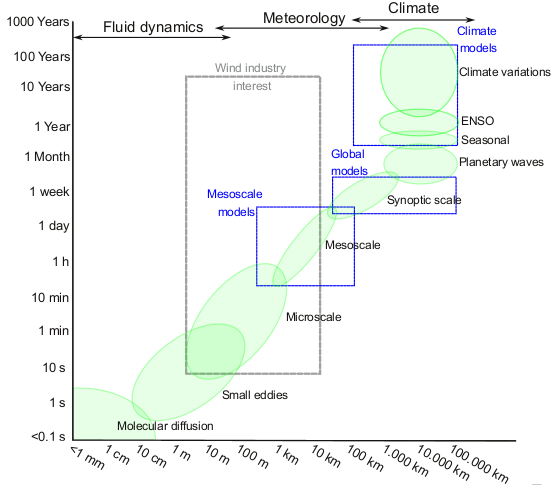
\includegraphics[width=0.7\linewidth]{Imagenes/terraincog}
\caption{Separación de escalas en simulación de mecánica de fluidos.}
\label{fig:terraincog}
\end{figure}


\section{ARW-WRF}
\subsection{Generalidades}
El modelo ARW-WRF (Advanced Research WRF) es un modelo no hidrostático que resuelve el sistema de ecuaciones para flujo compresible en su forma conservativa y utilizando una coordenada vertical de masa (o de presión hidrostática). Su coordenada vertical está definida como:
\begin{equation}
\eta = \frac{p_{dh}-p_{dht}}{\mu_d}
\end{equation}
Donde $p_{dh}$ corresponde a la componente hidrostática de la presión del aire seco, y:
\begin{equation}
\mu_d = p_{dhs} - p_{dht}
\end{equation}
es la masa de aire seco para una columna. En estas ecuaciones los subíndices $t$ y $s$ corresponden a los límites superior (top) e inferior (surface) del dominio. Las variables principales que resuelve el modelo son las velocidades covariantes $(u,v,w)$, masa de aire seco, geopotencial, temperatura potencial ($\theta$) y energía cinética turbulenta (TKE) de submalla (SGS). La ecuación de momentum, temperatura potencial, SGS TKE y otros escalares relevantes tienen una forma acoplada con la masa de aire seco, a priori:
\begin{equation}
\partial_t (\mu_d\theta) + \partial_x(\mu_d\mu\theta)+\partial_y(\mu_d\nu\theta)+\partial_\eta (\mu_d\omega\theta) = F
\end{equation}
Donde $F$ es la suma de la mezcla turbulenta junto con otras fuerzas y
\begin{equation}
\omega = d_t\eta
\end{equation}
es la velocidad en la coordenada vertical.

La discretización en el tiempo se realiza a través de un esquema de integración temporal múltiple. Este esquema separa los modos de alta frecuencia (i.e. ondas acústicas y de gravedad) de los modos de baja frecuencia (modo físico). ARW utiliza un esquema RK3 y durante cada paso en el RK, el modo de alta frecuencia que se propaga horizontalmente es integrado a través de un esquema \emph{forward-backward} utilizando un paso de tiempo acústico, que es típicamente un orden de magnitud mas pequeño que el paso físico, mientras que un esquema implícito es utilizado para el modo de alta frecuencia que se propaga de manera vertical.
\subsection{Ecuaciones Resueltas}
\subsection{Discretización Espacial}
\subsection{Discretización Temporal}
\subsection{Aspectos Numéricos}
\subsubsection{Advección}
\subsubsection{Difusión}
\subsubsection{Microfísicas}


\chapter{Caso de Estudio}
\section{Aspectos Generales}
Para este caso, se está interesado en caracterizar el comportamiento del viento en la zona costera de Valparaíso, mas específicamente en el sector de Laguna Verde, lugar donde existe un gran interés a causa de su alto potencial eólico, tal como lo explicita el Explorador Eólico de la Universidad de Chile y cuyo resultado se puede observar en la figura \ref{fig:explorador}.

\begin{figure}[H]
	\centering
	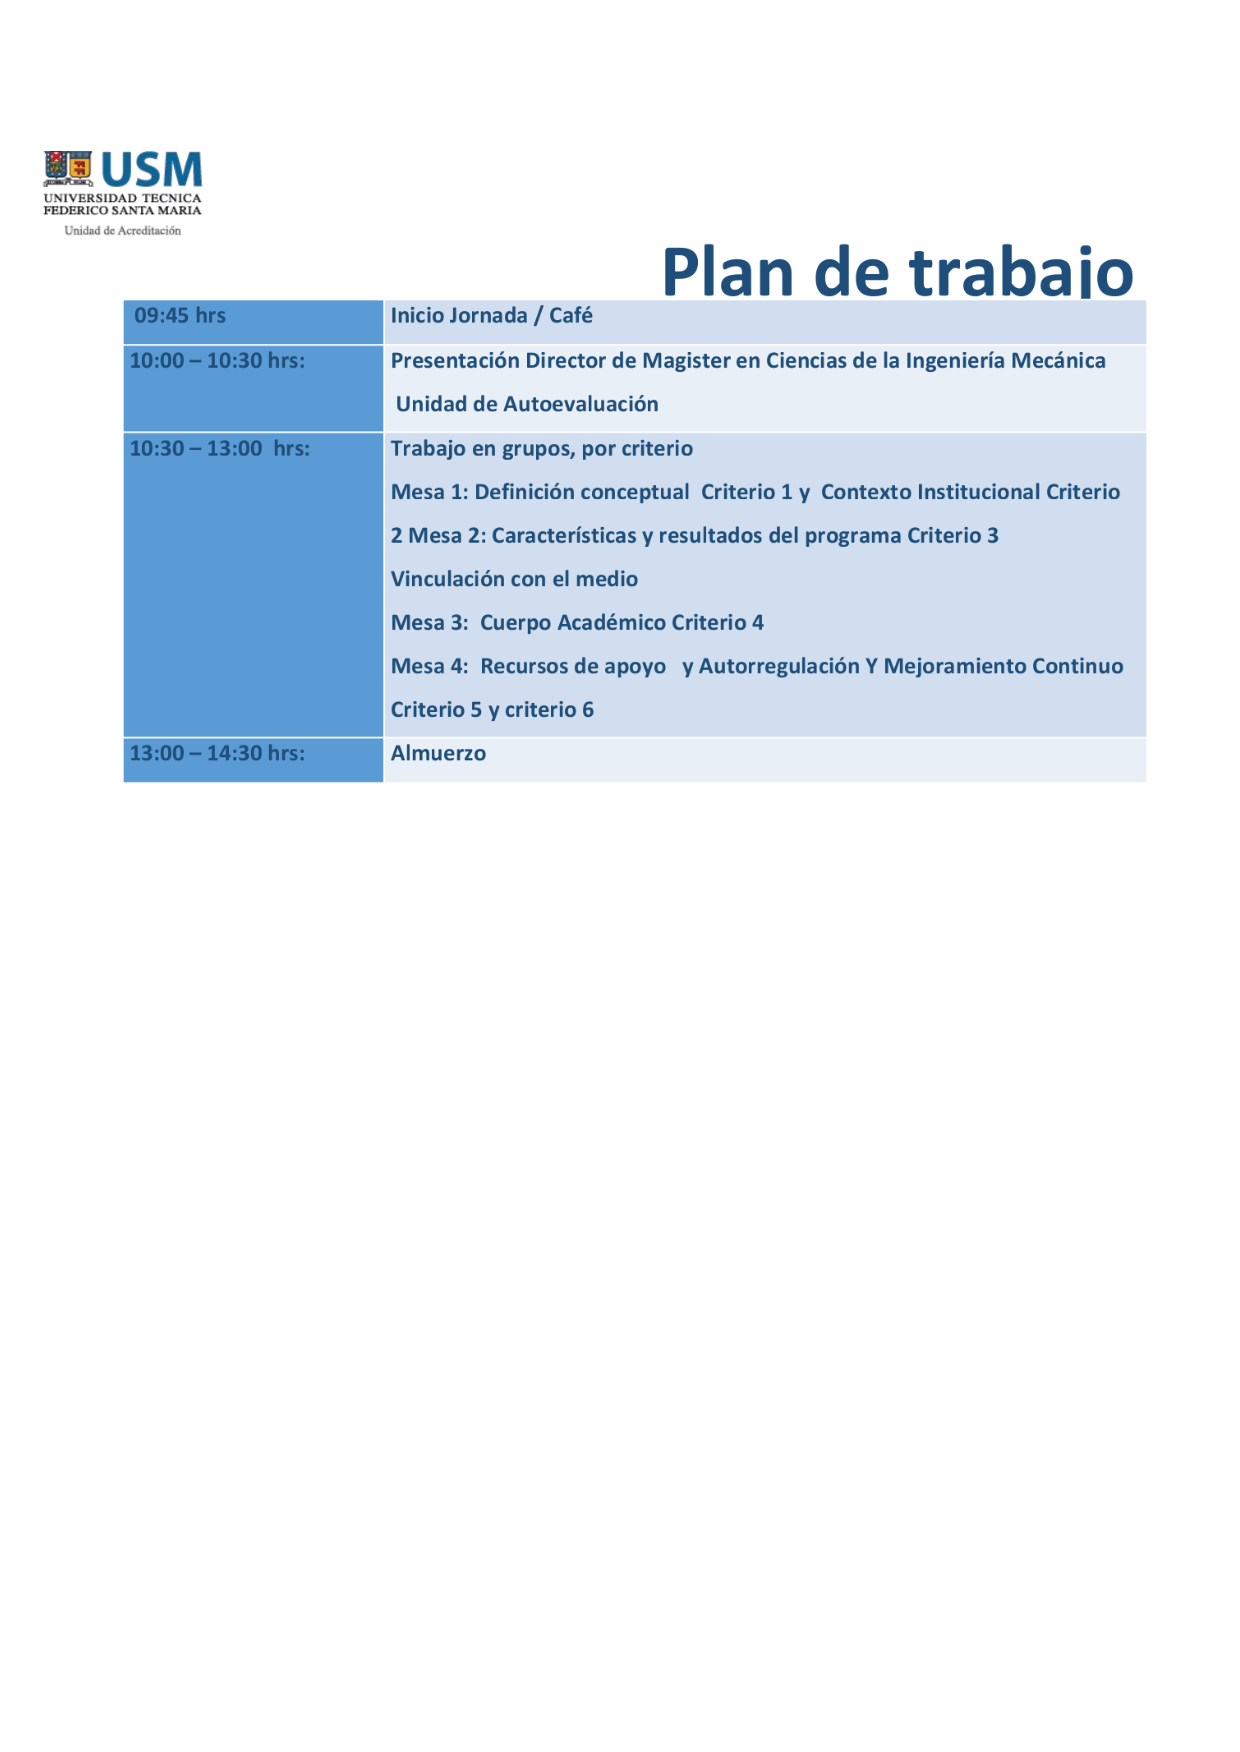
\includegraphics[width=0.9\linewidth,trim={5.4cm 2cm 15cm 5.5cm},clip]{Imagenes/explorador}
	\caption{Información del Explorador Eólico para la zona de interés.}
	\label{fig:explorador}
\end{figure}

Los datos de la figura \ref{fig:explorador} corresponde a un promedio anual para la magnitud de la velocidad en cada punto de la malla numérica. Esta malla tiene una resolución de 1 [km], la cual, si bien permite obtener información relevante acerca de zonas con alto potencial eólico, es ineficiente para capturar el comportamiento del flujo en el terreno complejo. Es por esto, que es relevante afinar la simulaciones aplicando técnicas modernas y apuntar a una mejor calidad para la caracterización eólica de una zona.

La simulación de la que trata este informe se realiza en un día standart del mes de Enero del año 2010. El día de simulación se escogió, por una parte, por las facilidades para obtener las condiciones de contorno provenientes de otros modelos y por otro, por que en verano existe un comportamiento mas energético del viento.
\section{Resolución Espacial}
Se discretiza espacialmente la zona en 6 dominios colocados de forma telescópica y centrados en el punto de coordenadas (-33.097344, -71730552) que corresponde a la costa de Punta Curaimilla.

Como el objetivo principal es obtener una malla fina con resolución de 50 [m], a la malla mas gruesa se le asigna un $\Delta x = \Delta y = 12150$ [m] y cada malla se va afinando en un factor de 3 su resolución. La resolución de malla mas gruesa es electa debido a su compatibilidad con la interpolación de las condiciones de borde del modelo global.

La distribución de las mallas y su proyección sobre la tierra se pueden observar en las figuras \ref{fig:0102}, \ref{fig:0203}, \ref{fig:0304}, \ref{fig:0405} y \ref{fig:0506}.

\begin{figure}[H]
	\centering
	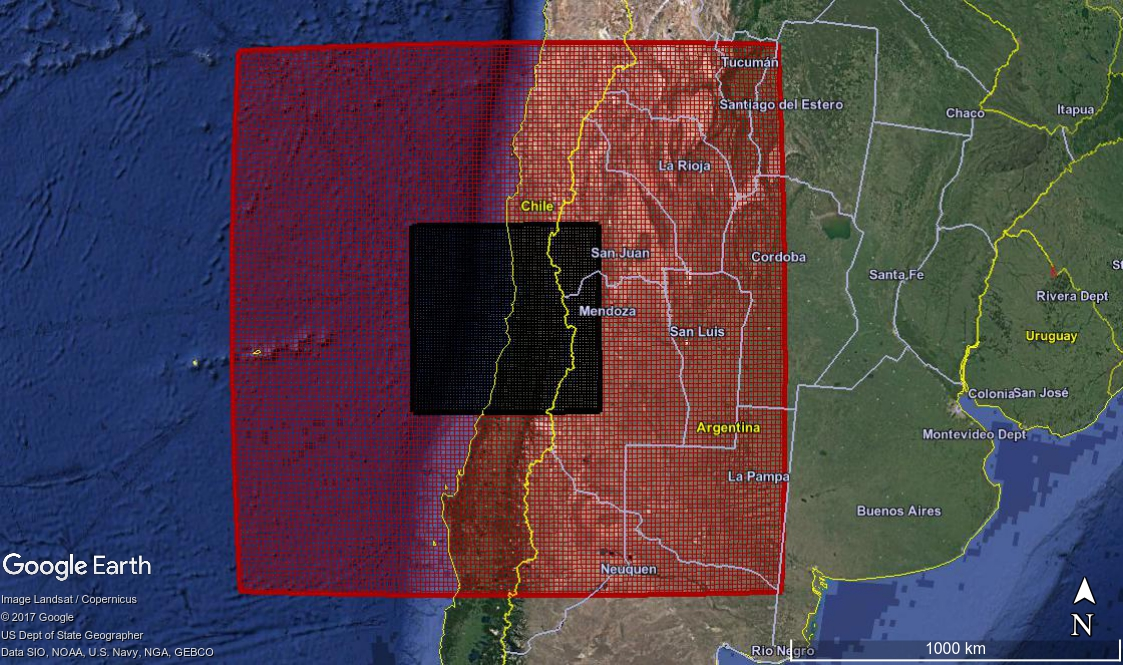
\includegraphics[width=0.95\linewidth]{Imagenes/d06d05}
	\caption{Dominios de las mallas exteriores d01 y d02.}
	\label{fig:0102}
\end{figure}

\begin{figure}[H]
	\centering
	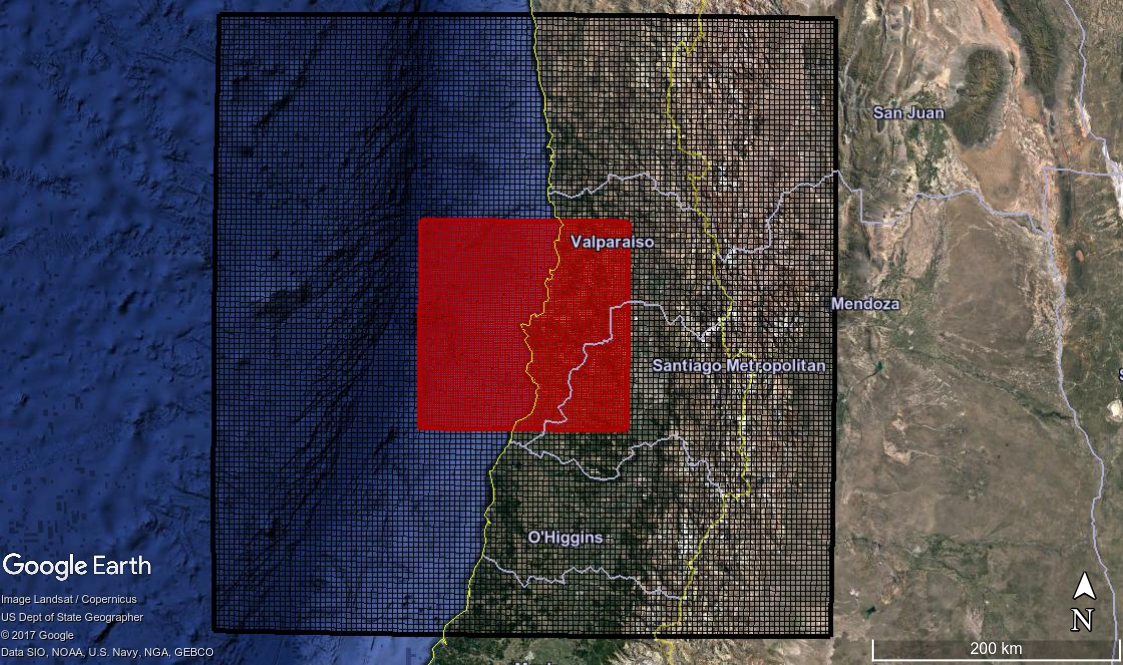
\includegraphics[width=0.95\linewidth]{Imagenes/d05d04}
	\caption{Dominios d02 y d03.}
	\label{fig:0203}
\end{figure}

\begin{figure}[H]
	\centering
	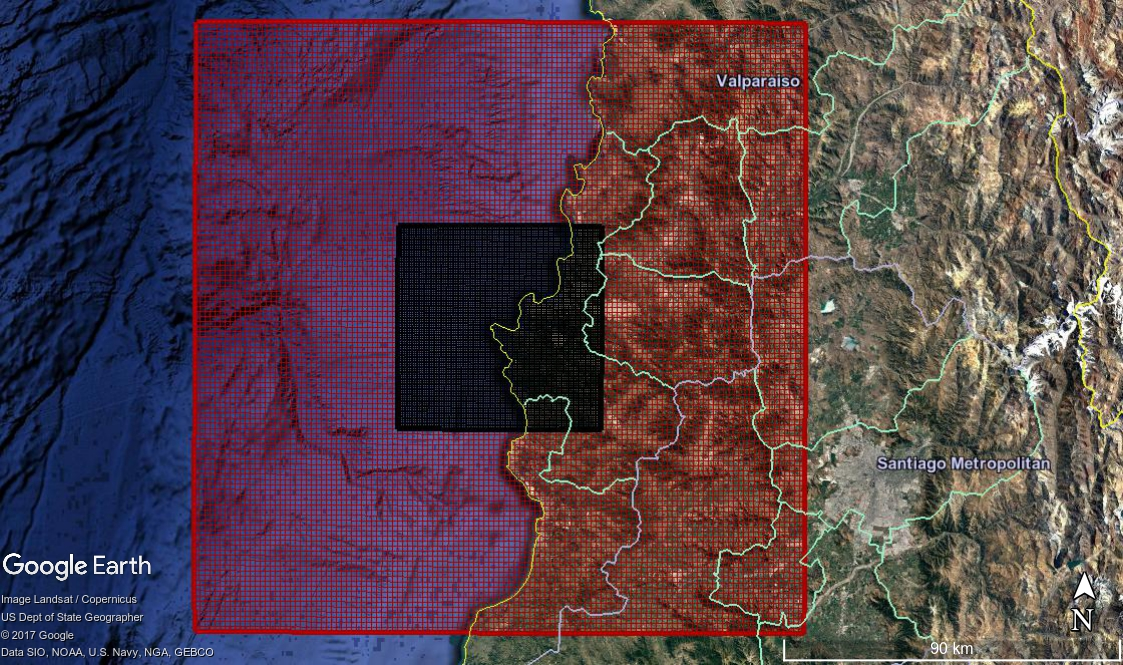
\includegraphics[width=0.95\linewidth]{Imagenes/d04d03}
	\caption{Dominios d03 y d04 (LES).}
	\label{fig:0304}
\end{figure}

\begin{figure}[H]
	\centering
	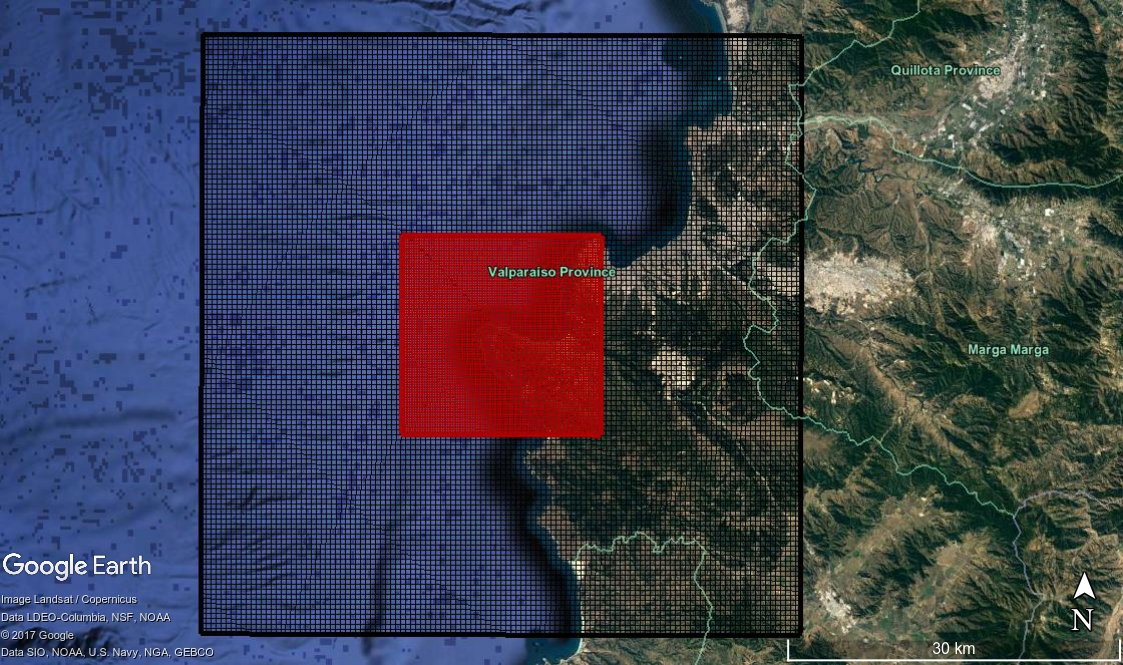
\includegraphics[width=0.95\linewidth]{Imagenes/d03d02}
	\caption{Dominios d04 (LES) y d05 (LES).}
	\label{fig:0405}
\end{figure}

\begin{figure}[H]
	\centering
	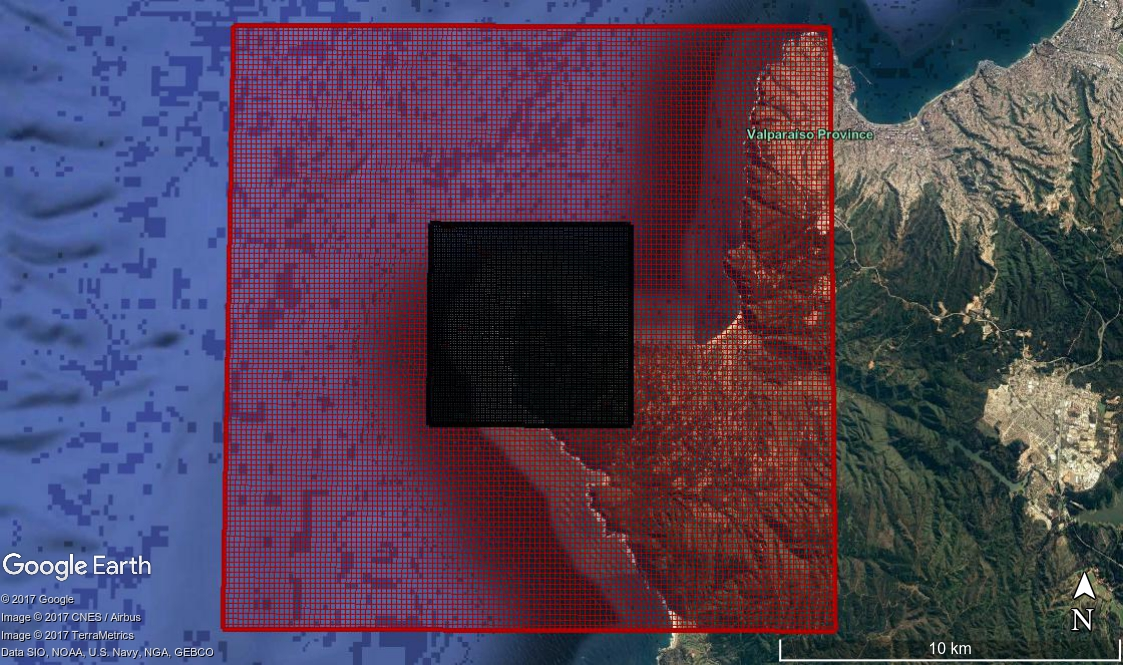
\includegraphics[width=0.95\linewidth]{Imagenes/d02d01}
	\caption{Dominios mas finos d05 (LES) y d06 (LES).}
	\label{fig:0506}
\end{figure}
Cada malla consta de $121\times 121$ nodos en el sentido horizontal y 47 nodos en sentido vertical. Existe un refinamiento de la malla en la cercanía a la superficie de modo de tener los 10 primeros niveles dentro de los primeros 300 [m] de atmósfera.
\section{Resolución Temporal}
Para la simulación se utiliza un paso de tiempo físico constante. Para no tener problemas de inestabilidades y que el modelo diverja, se opta por una relación empírica conservadora que es parte de las buenas prácticas en el uso del WRF. Se utiliza:
\begin{equation}
\Delta t \approx \Delta x
\end{equation}
Donde $\Delta x$ tiene unidades de [km]. Luego, el paso de tiempo para el dominio mas grande será $\Delta x=12$ [s] y este valor va reduciéndose 1/3 en cada dominio anidado. Utilizando este valor no se presentaron problemas en el desarrollo de las iteraciones.
\section{Condiciones de Borde}
Para inicializar el modelo y para proveer de información en los contornos cada 6 horas, se utilizan los datos de los análisis operacionales provenientes del modelo global GFS con resolución de $0.5^\circ$ ($\approx 55.6$ [km])

Por otra parte, como el dominio mas grande a simular cae dentro de lo que es una simulación de mesoescala y tomando en consideración las proyecciones debido a la curvatura de la tierra para esta zona en particular, se decide fijar la condición de borde superior para la coordenada vertical de presión a $p_{dht} = 5000$ [kPa] siguiendo la recomendación del manual del programa.
\section{Información del Terreno}
Debido a que los últimos 3 dominios son de 450, 150 y 50 [m] respectivamente en sus tamaños de malla, es necesario proveer al modelo información superficial de alta resolución. Para la topografía se utilizan los datos de la operación satelital SRTM de la NASA que tienen resolución de 3 segundos de arco. Para las propiedades de la superficie como vegetación, rugosidad, tipo de uso de suelo se utilizan los datos que provienen de los instrumentos satelitales MODIS.
\section{Parametrizaciones}
\begin{table}[h!]
	\caption{Esquemas de Parametrización Utilizados.}\label{tab:esquemas}
	\centering
	\begin{tabular}{lllllll}
		\toprule
		Física 					& d01	&	d02	&	d03	&	d04	&	d05	&	d06 \\
		\midrule
		Micro-físicas		 	& WSM 5-especie&d02&d02&d02&d02&d02  \\
		Cúmulos			 		& -- &d02&d02&d02&d02&d02\\ 
		Capa Superficial	 	& QNSE &d02&d02&d02&d02&d02\\
		PBL				 		& QNSE &d02&d02&d02&d02&d02\\
		Modelo de Suelo 		& 5 capas&d02&d02&d02&d02&d02 	\\
		Radiación Onda Larga	& RRTMG&d02&d02&d02&d02&d02 \\
		Radiación Onda Corta	& Dudhia&d02&d02&d02&d02&d02 \\
		\bottomrule
	\end{tabular}
\end{table}
\section{Monitoreo de Variables}